\section{测试}
在测试中,我首先比较了在50、100、150、200、250、300轮次中损失值和准确率的变化,可以发现在150-200轮次,损失值和准确率就开始不再变化。
\begin{figure}[H]
	\centering
	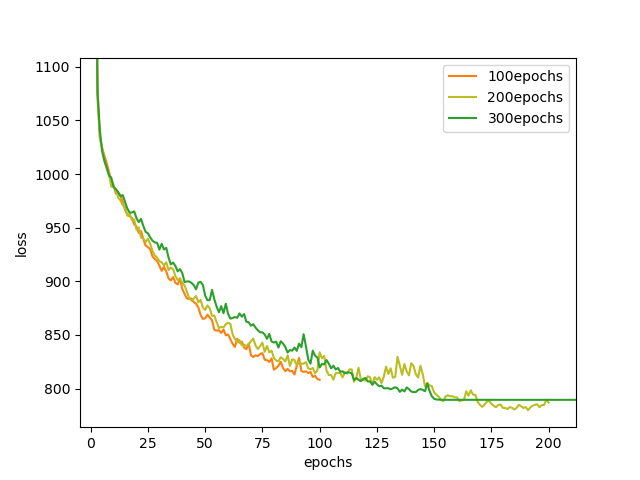
\includegraphics[width=0.7\textwidth]{loss3.png}
	\caption{损失值随训练轮次变化}
	\label{fig:example}
\end{figure}
\begin{figure}[H]
	\centering
	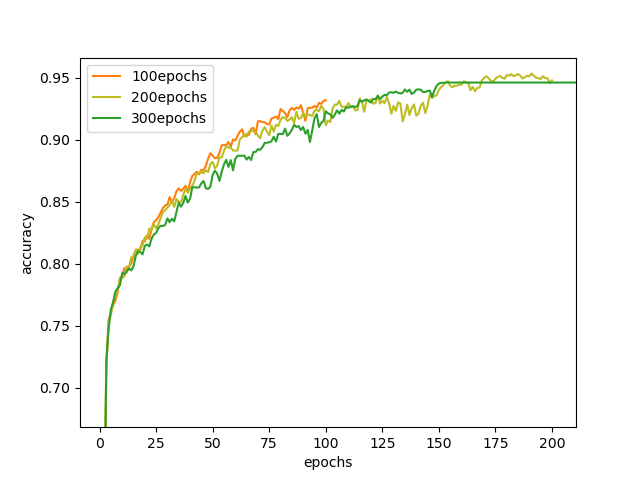
\includegraphics[width=0.7\textwidth]{acc3.png}
	\caption{准确率随训练轮次变化}
	\label{fig:example}
\end{figure}

\newpage
因此,我们将准确率的测试放在175次进行。结果如图所示。
\begin{figure}[H]
	\centering
	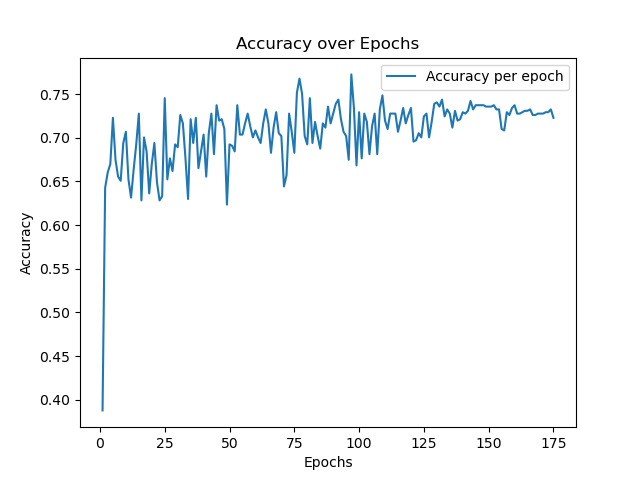
\includegraphics[width=0.7\textwidth]{accperepoch.png}
	\caption{175轮次准确率随轮次变化}
	\label{fig:example}
\end{figure}
从图片中可以看出,准确率在70\%上下徘徊,并不稳定,最后可能是收敛到72.5\%左右,相对来说并不高。模型还有很大的进步空间。
